% - [x] disclaimer, this is not new and based on all these sources. We order it slightly differently to work on GPUs so we will outline it here
% - [x] provide summary of integrator first then provide details. Then there's space in the first section to discuss details of the implementation
%  - [ ] How was this implemented on GPUs and what made it different
%    - [ ] what does Cholla do when I press go?
%      - [ ] allocations, data movement, etc
%  - [x] here's the details on all the math

\section{Methods}
\label{sec:methods}

Magnetic fields play a key role in many astrophysical phenomena, but are often neglected in numerical simulations due to the computational expense of magnetohydrodynamics. Part of this expense arises due to the wide range of temporal and physical scales over which magnetic field dynamos operate. Numerical integration of the MHD equations is also challenging; the additional waves compared to hydrodynamics and the requirement to maintain the divergence free condition result in considerable added complexity.

Given these considerations, MHD simulations often need to be both high resolution and use robust, divergence free methods, which tend to increase the computational cost. This limitation can be overcome by harnessing new GPU based supercomputers efficiently. Thus, we have elected to expand the existing massively parallel GPU-based hydrodynamics code, Cholla, to incorporate the effects of MHD. In this section we describe the equations solved and methods used by the MHD module of Cholla. While the algorithms themselves are not new, our particular choices are not laid out in any one reference, so we outline them all here. We also highlight choices that are particularly relevant to solving these equations on GPUs.

\subsection{Magnetohydrodynamics}
\label{sec:methods-mhd}

Cholla solves the ideal MHD equations in their conserved Eulerian form using a finite volume method \citep{Godunov}. These equations neglect all dissipative processes: finite viscosity, electrical resistivity and thermal conductivity. These approximations are reasonable when simulation regions of low density such as the ISM, CGM, and IGM. Although we also neglect these additional processes at present, our methods are fully compatible with a future expansion to include additional physics that depends on magnetic fields, such as anisotropic conduction or cosmic ray transport.

The ideal MHD equations are:

\begin{equation}
    \label{eqn:mass-conservation}
    \frac{\partial \rho}{\partial t} + \nabla \cdot (\rho \boldsymbol{v}) = 0
\end{equation}

\begin{equation}
    \label{eqn:momentum-conservation}
    \frac{\partial \rho\boldsymbol{v}}{\partial t} + \nabla \cdot (\rho \boldsymbol{v}\otimes\boldsymbol{v} - \boldsymbol{B}\otimes\boldsymbol{B} + P_T\boldsymbol{I}) = 0
\end{equation}

\begin{equation}
    \label{eqn:energy-conservation}
    \frac{\partial E}{\partial t} + \nabla \cdot ( (E + P_T) \boldsymbol{v} + \boldsymbol{B}(\boldsymbol{B}\cdot\boldsymbol{v}) ) = 0
\end{equation}

\begin{equation}
    \label{eqn:induction}
    \frac{\partial \boldsymbol{B}}{\partial t} - \nabla \times (\boldsymbol{v} \times \boldsymbol{B}) = 0
\end{equation}

\noindent where $\rho$ is density, $\boldsymbol{v} = ( v_x, v_y, v_z)$ is the velocity vector, $t$ is time, $\boldsymbol{B} = ( B_x, B_y, B_z)$ is the magnetic field, $\boldsymbol{I}$ is the identity tensor, $P_T \equiv P + \frac{1}{2}(\boldsymbol{B} \cdot \boldsymbol{B})$ is the total pressure, $E$ is the total energy per unit volume $E \equiv \epsilon + \frac{1}{2}\rho(\boldsymbol{v}\cdot\boldsymbol{v}) + \frac{1}{2}(\boldsymbol{B}\cdot\boldsymbol{B})$, and the units are such that magnetic permeability $\mu_0 = 1$. 

Equation \ref{eqn:mass-conservation} describes the conservation of mass, equation \ref{eqn:momentum-conservation} describes the conservation of momentum, equation \ref{eqn:energy-conservation} describes the conservation of energy, and equation \ref{eqn:induction} is the induction equation, which describes the divergence free condition. Cholla uses an ideal gas equation of state  which is $P \equiv \epsilon(\gamma - 1)$ where $\gamma$ is the adiabatic index and $\epsilon$ is the internal energy density. 

In practice these equations are used in their vector form, where $\boldsymbol{U}$ and $\boldsymbol{W}$ are the conserved and primitive variables respectively:

\begin{align}
    \boldsymbol{U} = \begin{bmatrix}
            \rho &
            v_x &
            v_y &
            v_z &
            E   &
            B_x &
            B_y &
            B_z
         \end{bmatrix}
    \\
    \boldsymbol{W} = \begin{bmatrix}
            \rho &
            v_x &
            v_y &
            v_z &
            P   &
            B_x &
            B_y &
            B_z 
         \end{bmatrix}
\end{align}

The conservation equations, in Cartesian coordinates, can then be rewritten as

\begin{equation}
    \label{eqn:vector-conserved}
    \frac{\partial \boldsymbol{U}}{\partial t} + 
    \frac{\partial \boldsymbol{F_x}}{\partial x} + 
    \frac{\partial \boldsymbol{F_y}}{\partial y} + 
    \frac{\partial \boldsymbol{F_z}}{\partial z} = 0 
\end{equation}

where $\boldsymbol{F_x}$, $\boldsymbol{F_y}$, and $\boldsymbol{F_z}$ are the vectors of fluxes in the $x$, $y$, and $z$ direction respectively and are given by

\begin{equation}
    \boldsymbol{F_x} = \begin{bmatrix}
            \rho v_{x} \\
            \rho v_{x}^2 + P_{T} - B_{x}^2 \\
            \rho v_{x} v_{y} - B_{x} B_{y} \\
            \rho v_{x} v_{z} - B_{x} B_{z} \\
            v_{x} \left( E + p_{T} \right) - B_{x} \left( \boldsymbol{v} \cdot \boldsymbol{B} \right) \\
            0 \\
            B_{y} v_{x} - B_{x} v_{y} \\
            B_{z} v_{x} - B_{x} v_{z} \\
         \end{bmatrix}
\end{equation}

\begin{equation}
    \boldsymbol{F_y} = \begin{bmatrix}
            \rho v_{y} \\
            \rho v_{y} v_{x} - B_{y} B_{x} \\
            \rho v_{y}^2 + P_{T} - B_{y}^2 \\
            \rho v_{y} v_{z} - B_{y} B_{z} \\
            v_{y} \left( E + P_{T} \right) - B_{y} \left( \boldsymbol{v} \cdot \boldsymbol{B} \right) \\
            B_{x} v_{y} - B_{y} v_{x} \\
            0 \\
            B_{z} v_{y} - B_{y} v_{z} \\
         \end{bmatrix}
\end{equation}

\begin{equation}
    \boldsymbol{F_z} = \begin{bmatrix}
            \rho v_{z} \\
            \rho v_{z} v_{x} - B_{z} B_{x} \\
            \rho v_{z} v_{y} - B_{z} B_{y} \\
            \rho v_{z}^2 + P_{T} - B_{z}^2 \\
            v_{z} \left( E + P_{T} \right) - B_{z} \left( \boldsymbol{v} \cdot \boldsymbol{B} \right) \\
            B_{x} v_{z} - B_{z} v_{x} \\
            B_{y} v_{z} - B_{z} v_{y} \\
            0
         \end{bmatrix}.
\end{equation}

Some other useful MHD equations are given in Appendix \ref{appen:mhd-glossary} such as the eigenvalues, wave speeds, etc.



\subsection{Overview of the VL+CT Integrator}
\label{sec:vlct-summary}

To integrate these equations in Cholla, we use the VL+CT (Van Leer plus Constrained Transport) integrator introduced in \cite{stone_2009}, along with the HLLD Riemann solver from \cite{hlld_2005}. The specific algorithm is from \cite{stone_2009} with some clarifying details from \cite{gardiner_2005,gardiner_unsplit_2008,stone_athena_2008} and the piecewise parabolic method is from \cite{felker_2018}. The VL+CT integrator is very similar in structure to the Van Leer integrator \citep{van_leer_2003, falle_1991, Toro}, though with significant new additions for Constrained Transport (CT). We note that this is now the default integrator used in Cholla, as we have found it to be more robust than the CTU algorithm described in \cite{schneider_2015}.

Constrained transport treats the magnetic field as a surface averaged quantity centered at cell interfaces rather than a volume averaged, cell centered quantity like the hydro variables; i.e. a staggered grid. Each face stores only the magnetic field perpendicular to that face, i.e. the $x,i+1/2,j,k$ face stores the $B_{x,i+1/2,j,k}$ magnetic field. At each time step, the magnetic field is then updated using edge averaged electric fields (Electromotive Force) computed from the magnetic flux returned by the Riemann solver. Updating the magnetic field with the electric field automatically fulfill the divergence free condition for magnetic fields, assuming that the initial conditions are divergence free.

A brief overview of the algorithm for a single time step using the VL+CT integrator is as follows; more detailed discussion of each step is presented in section \ref{vlct:header}.

\begin{enumerate}
    \item Compute the time step, $\Delta t$.
    \item Reconstruct interface states using a piecewise constant method (PCM) approximation.
    \item Solve the Riemann problem on every interface using the PCM interface states.
    \item Compute the edge centered electric fields.
    \item Update the $t=n$ conserved variables to $t=n+\Delta t/2$ using the computed fluxes and electric fields.
    \item Reconstruct interface states using a piecewise linear method (PLM) or piecewise parabolic method (PPM) approximation.
    \item Solve the Riemann problem on every interface using the higher order reconstructed interface states.
    \item Recompute the edge centered electric fields.
    \item Update the $t=n$ conserved variables to $t=n+\Delta t$ using the half time step fluxes and electric fields
\end{enumerate}

% ===========================================================================
\subsection{VL+CT Integrator in Detail}
\label{vlct:header}

\subsubsection{Step 1: Compute the Time Step}
\label{vlct:dt}

The first step is to compute the time step. This it the minimum crossing time of any wave in any cell multiplied by a Courant factor to maintain the Courant–Friedrichs–Lewy condition \cite{cfl}.

\begin{equation}
    \begin{aligned}
        \label{eqn:dt}
        \Delta t = C_{CFL} \min \left(
            \frac{\Delta x}{\mid v^n_{x,i,j,k} \mid + C^n_{f,i,j,k}}, \right. \\ \left.
            \frac{\Delta y}{\mid v^n_{y,i,j,k} \mid + C^n_{f,i,j,k}}, 
            \frac{\Delta z}{\mid v^n_{z,i,j,k} \mid + C^n_{f,i,j,k}}
        \right).
    \end{aligned}
\end{equation}

\noindent where $\Delta t$ is the time step, $C_{CFL} \leq 0.5$ is the CFL number, $\mid v^n_{l,i,j,k}\mid $ is the magnitude of the velocity in the $l$ direction velocity in the ${i,j,k}$ cell, and $c^n_f $ is the fast magnetosonic wave-speed computed using \emph{cell centered} values. The fast and slow magnetosonic speeds are

\begin{equation}
    c_{f,s} = \sqrt{\frac
    {\gamma p + \mid \boldsymbol{B} \mid^2 \pm \sqrt{\left( \gamma p \;+ \mid \boldsymbol{B} \mid^2 \right)^2 - 4\gamma p B_x^2 } }
    {2\rho}}
\end{equation}

\noindent where the $+$ option corresponds to the fast magnetosonic speed, and $-$ to the slow.

Equation \ref{eqn:dt} computes the minimum crossing time of a wave in a specific cell and then a global reduction is performed to find the minimum in the entire grid; that minimum is used as the time step $\Delta t$. This reduction is done primarily on the GPU followed by an MPI ALL\_REDUCE. GPU reductions are complex and their performance is extremely sensitive to the method used, details of our reduction method are discussed in section \ref{sec:gpu-vs-cpu}. 

The cell-centered magnetic field is computed with a direct average of the face centered values:
\begin{equation}
    \begin{aligned}
        B^n_{x,i,j,k,} = \frac{1}{2} \left( B^n_{x,i+1/2,j,k} + B^n_{x,i-1/2,j,k} \right) \\
        B^n_{y,i,j,k,} = \frac{1}{2} \left( B^n_{y,i,j+1/2,k} + B^n_{y,i,j-1/2,k} \right) \\
        B^n_{z,i,j,k,} = \frac{1}{2} \left( B^n_{z,i,j,k+1/2} + B^n_{z,i,j,k-1/2} \right) \\
    \end{aligned}
\end{equation}
These cell-centered values for the magnetic field are used several times throughout the integrator. In CPU-based codes it is typically more efficient to compute these cell centered magnetic fields once and save them, since CPU-based codes are typically compute limited. Cholla is generally limited instead by GPU memory, so we recompute the cell-centered values when they are needed rather than permanently allocating the associated memory.



\subsubsection{Step 2: First Order Reconstruction}
\label{vlct:first-order-reconstruction}

Reconstructing the interface states at first order, or the piecewise constant method (PCM), is done by setting the primitive interface states values to the same value as the cell:

\begin{equation}
    \boldsymbol{W}_{L, i+1/2} = \boldsymbol{W}_{R, i-1/2} = \boldsymbol{W}_{i}
\end{equation}

\noindent where $ \boldsymbol{W}_{L/R, i\pm1/2} $ is the state on the left or right side of the cell. Even though Cholla only stored the conserved variables, the primitive variables are used for every reconstruction since the Riemann solver requires them. In higher order reconstructions we use the characteristic variables derived from the primitive variables.

Although PCM is too diffusive to be used on its own in both reconstruction steps it is excellent for debugging. We use it here as a computationally-inexpensive way to calculate first-order fluxes, which will be used for the ``predictor" step of this predictor-corrector algorithm. Most higher order methods revert to PCM near large discontinuities.

\subsubsection{Step 3: First Riemann Solve}
\label{vlct:first-riemann-solve}

The next step is to solve the Riemann problem with the first order interface states. We use the HLLD Riemann solver introduced in \cite{hlld_2005}. The longitudinal magnetic field does not require reconstruction and can be used directly since it is stored at the face. The transverse fields (i.e. the fields parallel to the interface) are reconstructed from the cell centered average (computed as shown in section \ref{vlct:dt}), then reconstructed using PCM identically to other fields.

The magnetic fluxes returned by the Riemann solver are the face centered electric fields \citep[see section 5.3 of][]{stone_athena_2008}. For clarity, we list in Table \ref{table:emf} the correlation between flux and electric field.

\begin{deluxetable*}{llll}
    \label{table:emf}
    \tablecaption{Magnetic Flux to Face Centered electric field}

    \tablehead{\colhead{HLLD Solve Direction} & \colhead{Equation for Magnetic Flux} & \colhead{Eqn. as a Cross Product} & \colhead{electric field}}

    \startdata
    $ X $ & $ V_x B_y - B_x V_y $ & $  (V \times B)_z $ & $ -\varepsilon_z $ \\ \hline
    $ X $ & $ V_x B_z - B_x V_z $ & $ -(V \times B)_y $ & $  \varepsilon_y $ \\ \hline
    $ Y $ & $ V_x B_y - B_x V_y $ & $  (V \times B)_z $ & $ -\varepsilon_x $ \\ \hline
    $ Y $ & $ V_x B_z - B_x V_z $ & $ -(V \times B)_y $ & $  \varepsilon_z $ \\ \hline
    $ Z $ & $ V_x B_y - B_x V_y $ & $  (V \times B)_z $ & $ -\varepsilon_y $ \\ \hline
    $ Z $ & $ V_x B_z - B_x V_z $ & $ -(V \times B)_y $ & $  \varepsilon_x $ \\ \hline
    \enddata

    \tablecomments{The directions used here are relative to the internal workings of the HLLD solver. Since the HLLD solver is inherently 1D we run it once for each of the faces of a cell. So in the case where the solver is running in the Y direction the solver's Y field is actually the Z field and the solvers Z field is actually the X field, cyclically extended for the Z direction}
\end{deluxetable*}

\subsubsection{Step 4: Compute the Constrained Transport Electric Field}
\label{vlct:emf}

The next step is to calculate the constrained transport electric field. These fields are \emph{line averaged} along each cell vertex. These line averaged fields are constructed by averaging the face centered electric fields from the previous step, and their slopes.

Example for computing the CT electric field in the $ z $-direction. The equations for computing the other directions are obtained by substituting out the $ z $ index with $ x $ or $ y $ and changing the derivatives appropriately.

\begin{equation}
    \label{eqn:emf-edge}
    \begin{aligned}
        \mathcal{E}_{z, i-1/2, j-1/2, k} = \frac{1}{4} \left(
              \mathcal{E}_{z, i-1/2, j, k}
            + \mathcal{E}_{z, i, j-1/2, k}
            + \mathcal{E}_{z, i-1/2, j-1, k}
            + \mathcal{E}_{z, i-1, j-1/2, k}\right) \\
        + \frac{\Delta y}{8} \left( \left( \frac{\partial \mathcal{E}_z }{\partial y} \right)_{i-1/2, j-1/4, k} + \left(  \frac{\partial \mathcal{E}_z }{\partial y} \right)_{i-1/2, j-3/4, k} \right) \\
        + \frac{\Delta x}{8} \left( \left( \frac{\partial \mathcal{E}_z }{\partial x} \right)_{i-1/4, j-1/2, k} + \left(  \frac{\partial \mathcal{E}_z }{\partial x} \right)_{i-3/4, j-1/2, k} \right)
    \end{aligned}
\end{equation}

$\mathcal{E}_{z, i-1/2, j-1/2, k}$ is the line averaged electric field, the firs four terms are the face averaged electric fields, and the four derivative terms are the derivatives of those fields in the direction towards the edge, details of which are in Equation \ref{eqn:emf-slope}. Figure \ref{fig:emf-graph} shows the spatial relationships between the derivatives and the relevant edge states and reference fields. Each edge requires 4 derivatives and they are computed as differences between a reference state and an edge state.

Technically, constrained transport uses the magnetic flux as the conservative variable and EMF (ElectroMotive Force) to update it. However, those values only differ from the magnetic flux density (i.e. the magnetic field) and the electric field respectively by factors of unit length we can treat them as the same thing, the same way we treat density and mass as the same for the hydro fields \cite{stone_athena_2008}. As such we use the magnetic field and electric field to evolve the grid. Electric fields have the proper units to evolve the magnetic flux density, $ B $, whereas EMF has the proper units to evolve the magnetic flux.

On any face there are two non-zero electric fields; both transverse to the face. The component that is used to calculate the field along a given edge is the component that is parallel to that edge; i.e. if the edge points along the $ z $-direction then the field pointing along the $ z $-direction is used, not the field in the $ x $ or $ y $ direction.

The derivatives from Equation \ref{eqn:emf-edge} are computed using the upwinded slope as follows

\begin{equation}
    \label{eqn:emf-upwind-slope}
    \left( \frac{\partial \mathcal{E}_z }{\partial y} \right)_{i-1/2, j-1/4, k} =
        \begin{cases}
            \left( \frac{\partial \mathcal{E}_z }{\partial y} \right)_{i-1, j-1/4, k} & \text{for} \; v_{x, i-1/2} > 0
            \\
            \\
            \left( \frac{\partial \mathcal{E}_z }{\partial y} \right)_{i, j-1/4, k} & \text{for} \; v_{x, i-1/2} < 0
            \\
            \\
            \frac{1}{2} \left( \left( \frac{\partial \mathcal{E}_z }{\partial y} \right)_{i-1, j-1/4, k} + \left( \frac{\partial \mathcal{E}_z }{\partial y} \right)_{i, j-1/4, k} \right) & \text{otherwise}
            \\
            \\
        \end{cases}
\end{equation}

where, for example, the derivatives are given by

\begin{equation}
    \label{eqn:emf-slope}
    \left( \frac{\partial \mathcal{E}_z }{\partial y} \right)_{i, j-1/4, k} =
    2 \left( \frac{\mathcal{E}_{z,i,j-1/2,k} - \mathcal{E}_{z,i,j,k}^{ref}}{\Delta y} \right).
\end{equation}

The $\mathcal{E}_{z,i,j,k}^{ref}$, is the cell centered reference field. This reference field can be computed with the following cross product

\begin{equation}
    \mathcal{E}_{i,j,k}^{ref,n} = - \left( \boldsymbol{v}^{n}_{i.j.k} \times \boldsymbol{B}^{n}_{i.j.k} \right).
\end{equation}

\begin{figure*}[ht!]
    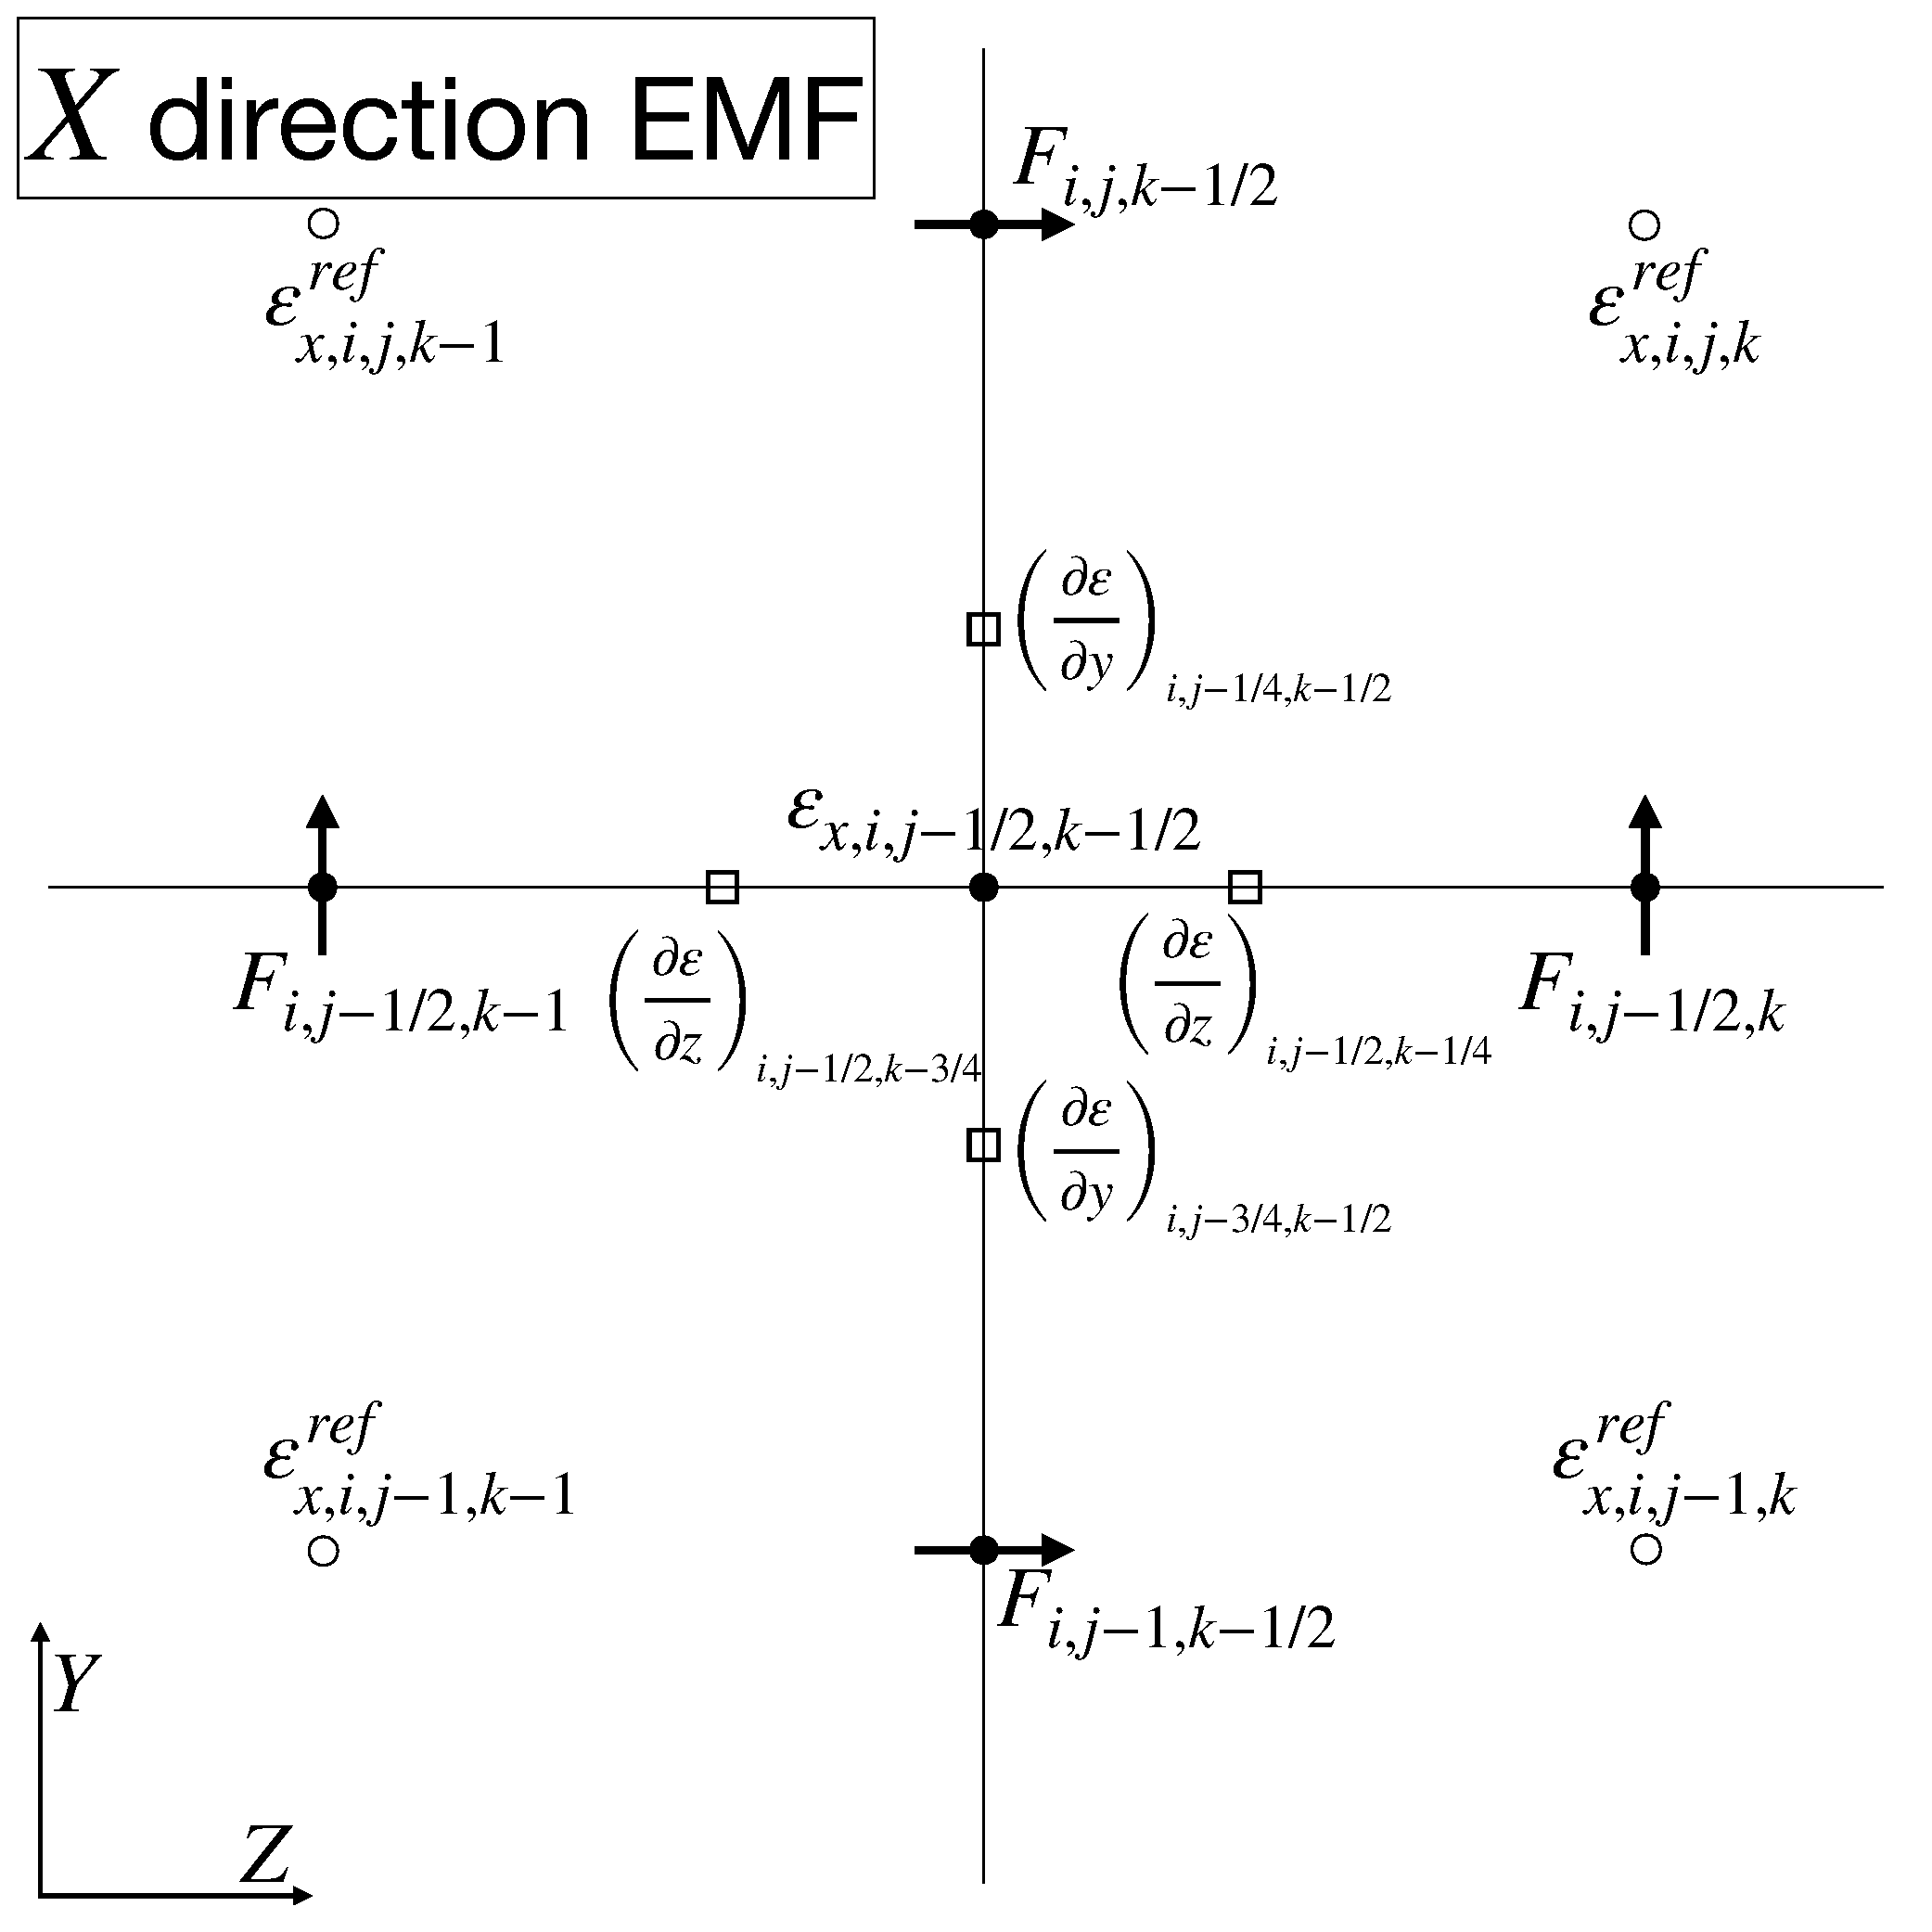
\includegraphics[width=0.32\linewidth]{assets/2-methods/CT-edge-field-figures-X.pdf}
    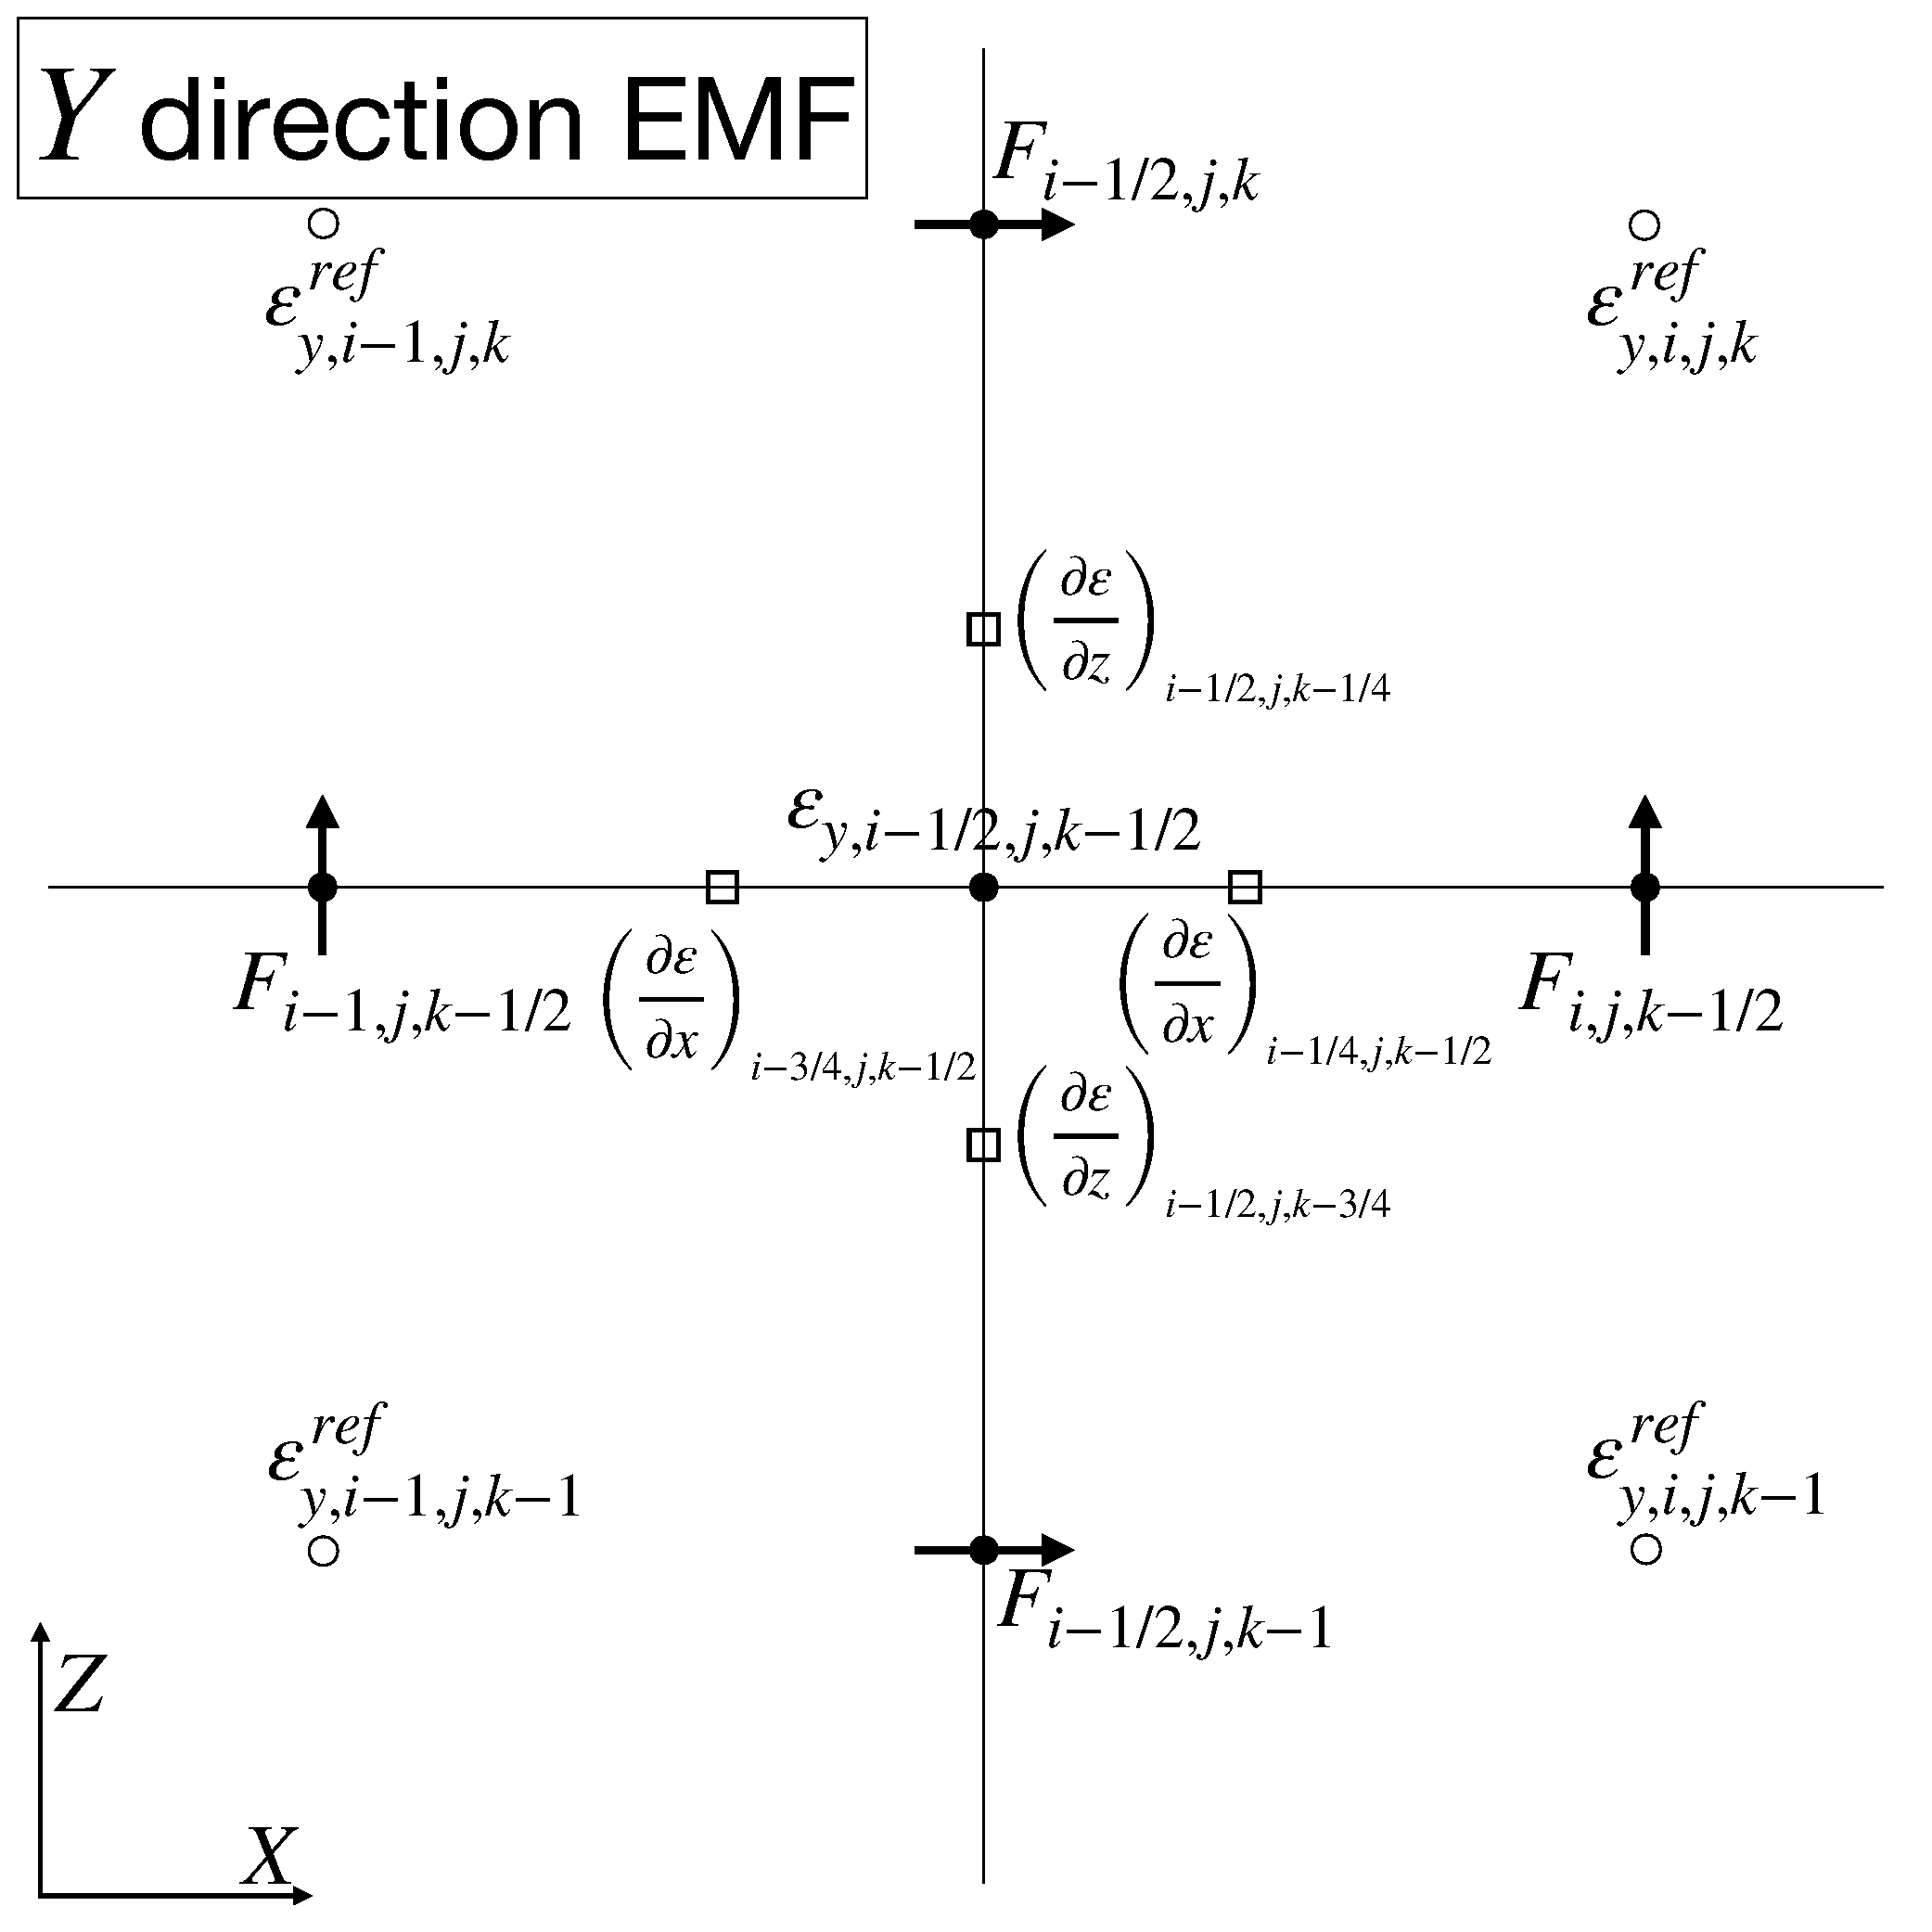
\includegraphics[width=0.32\linewidth]{assets/2-methods/CT-edge-field-figures-Y.pdf}
    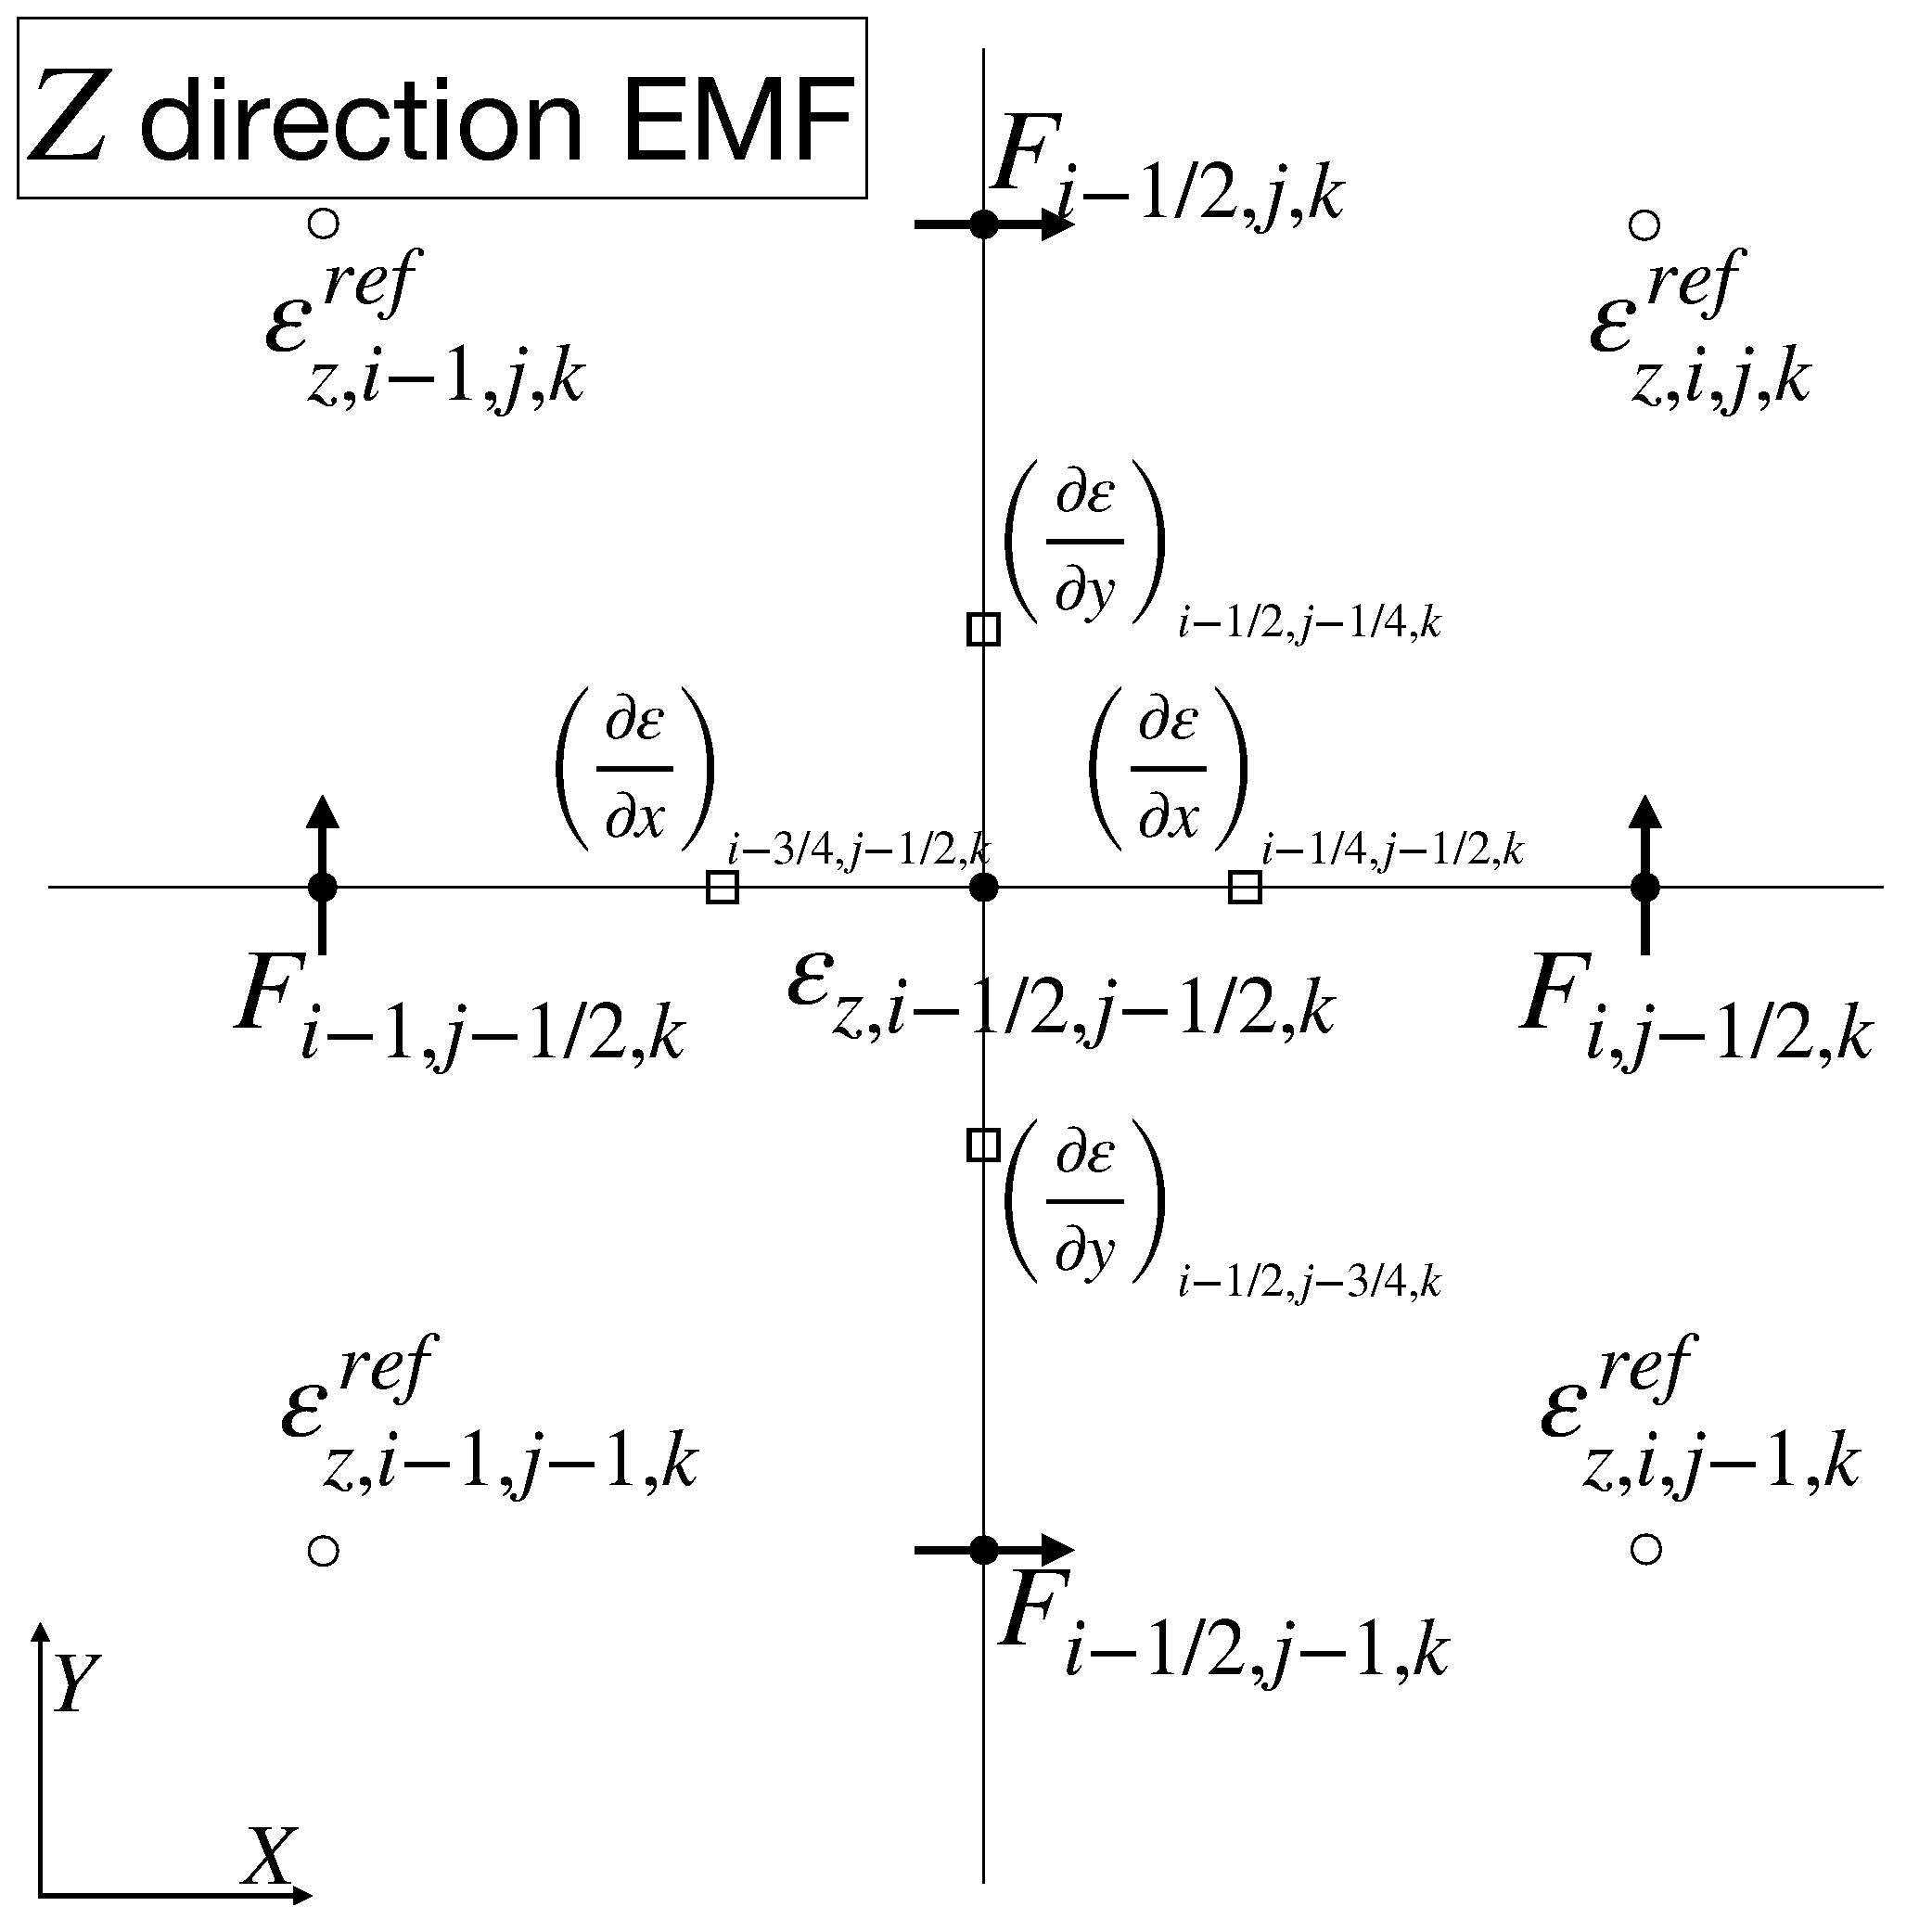
\includegraphics[width=0.32\linewidth]{assets/2-methods/CT-edge-field-figures-Z.pdf}
    \caption{2D slices in all three planes showing the location of the fluxes, edge electric fields, and derivatives. Based on Figure 5 of \cite{stone_athena_2008}.}
    \label{fig:emf-graph}
\end{figure*}

\subsubsection{Step 5. Perform the Half Time-step Update}
\label{vlct:half-dt-update}

Update the density, momenta, and energy, but not the magnetic fields, using the standard conservative update equation and the first-order fluxes from Step 3:

\begin{equation}
    \begin{aligned}
        \boldsymbol{U}^{n+1/2}_{i,j,k} = \boldsymbol{U}^{n}_{i,j,k}
        - \frac{\Delta t}{\Delta x} \left( \boldsymbol{F}^n_{x,i+1/2,j,k} - \boldsymbol{F}^n_{x,i-1/2,j,k} \right) \\
        - \frac{\Delta t}{\Delta y} \left( \boldsymbol{F}^n_{y,i+1/2,j,k} - \boldsymbol{F}^n_{y,i-1/2,j,k} \right) \\
        - \frac{\Delta t}{\Delta z} \left( \boldsymbol{F}^n_{z,i+1/2,j,k} - \boldsymbol{F}^n_{z,i-1/2,j,k} \right).
    \end{aligned}
\end{equation}

Update the magnetic field using the electric fields computed in Step 4:

\begin{equation}
    \begin{aligned}
        B^{n+1/2}_{x,i-1/2,j,k} = B^{n}_{x,i-1/2,j,k}
        + \frac{\Delta t}{\Delta z} \left( \mathcal{E}^n_{y,i-1/2,j,k+1/2} - \mathcal{E}^n_{y,i-1/2,j,k-1/2} \right) \\
        - \frac{\Delta t}{\Delta y} \left( \mathcal{E}^n_{z,i-1/2,j+1/2,k} - \mathcal{E}^n_{z,i-1/2,j-1/2,k} \right)
    \end{aligned}
\end{equation}

\begin{equation}
    \begin{aligned}
        B^{n+1/2}_{y,i,j-1/2,k} = B^{n}_{y,i,j-1/2,k}
        + \frac{\Delta t}{\Delta x} \left( \mathcal{E}^n_{z,i+1/2,j-1/2,k} - \mathcal{E}^n_{z,i-1/2,j-1/2,k} \right) \\
        - \frac{\Delta t}{\Delta z} \left( \mathcal{E}^n_{x,i,j-1/2,k+1/2} - \mathcal{E}^n_{x,i,j-1/2,k-1/2} \right)
    \end{aligned}
\end{equation}

\begin{equation}
    \begin{aligned}
        B^{n+1/2}_{z,i,j,k-1/2} = B^{n}_{z,i-1/2,j,k}
        + \frac{\Delta t}{\Delta y} \left( \mathcal{E}^n_{x,i,j+1/2,k-1/2} - \mathcal{E}^n_{x,i,j-1/2,k-1/2} \right) \\
        - \frac{\Delta t}{\Delta x} \left( \mathcal{E}^n_{y,i+1/2,j,k-1/2} - \mathcal{E}^n_{y,i-1/2,j,k-1/2} \right).
    \end{aligned}
\end{equation}

\subsubsection{Step 6. Half Time-step Second Order Reconstruction}
\label{vlct:higher-order-reconstruction}

Step 5 results in first order time-averaged values for the cell-centered conserved variables and face-centered magnetic fields. To make the integration second-order in time, we need to perform a ``corrector" step. First, weperform a higher order interface reconstruction. The method shown here is for Piecewise Linear Method (PLM), reconstruction. Cholla currently implements piecewise constant, piecewise linear, and piecewise parabolic reconstruction, with limiting in the characteristic variables, for MHD. The piecewise parabolic method that Cholla utilizes is discussed in detail in \cite{felker_2018}. Using the third order piecewise parabolic method for spatial reconstruction does typically give slightly more accurate results at a given resolution compared to PLM, but since the method is formally second order it does not improve the overall order of convergence.

Note that at a given face only the transverse components of the electric field need to be reconstructed. The longitudinal component is already given at the face.

\begin{enumerate}
    \item Compute the primitive variables
    
    \item Compute the left, right, centered, and Van Leer differences in the primitive variables
    \begin{align} 
        \delta \boldsymbol{W}_{L,i} = \boldsymbol{W_{i}} - \boldsymbol{W_{i-1}} \\ 
        \delta \boldsymbol{W}_{R,i} = \boldsymbol{W_{i+1}} - \boldsymbol{W_{i}} \\
        \delta \boldsymbol{W}_{C,i} = \frac{\boldsymbol{W_{i+1}} - \boldsymbol{W_{i-1}}}{2} \\
        \delta \boldsymbol{W}_{VL,i} = 
        \begin{cases}
            \frac{2 \boldsymbol{W}_{L,i} \boldsymbol{W}_{R,i}}{\boldsymbol{W}_{L,i} +\boldsymbol{W}_{R,i}} ,& \text{if } \boldsymbol{W}_{L,i} \boldsymbol{W}_{R,i} > 0\\
            0,              & \text{otherwise}
        \end{cases}
    \end{align}
    
    \item Project the slopes into the characteristic variables, $\boldsymbol{a}$, using the eigenvectors given in the appendix of \cite{stone_athena_2008}. Note that to maintain mathematical consistency we use the eigenvectors of the $\boldsymbol{w_{i}}$ cell for all four slopes and the later projection back to primitive variables.
    \item Apply monotonicity constraints to the characteristic differences to ensure that the reconstruction is total variation diminishing (TVD). We use the following limiter, given in \cite{leveque2002finite}.
    \begin{equation}
        \label{eqn:limiter}
        \delta \boldsymbol{a}_{m,i} = 
        \begin{cases}
             \text{sgn}(\boldsymbol{a}_{C,i})\min(2\abs{\boldsymbol{a}_{L,i}},2\abs{\boldsymbol{a}_{R,i}},\abs{\boldsymbol{a}_{C,i}},\abs{\boldsymbol{a}_{VL,i}}),& \text{if } \boldsymbol{a}_{L,i} \boldsymbol{a}_{R,i} > 0\\
            0,              & \text{otherwise}
        \end{cases}
    \end{equation}
    \item Project the limited characteristic slopes, $\delta \boldsymbol{a}_{m}$, back into the primitive variables, $\delta \boldsymbol{W}_{m}$, using the eigenvectors given in \cite{stone_athena_2008}.
    \item Compute the interface states $\boldsymbol{W}_{L, i+1/2}$ and $\boldsymbol{W}_{R, i-1/2}$:
\end{enumerate}

    \begin{equation}
        \begin{aligned}
            \boldsymbol{W}_{L, i+1/2} = \boldsymbol{W}_{i} + \frac{\delta \boldsymbol{W}_{m, i}}{2} \\
            \boldsymbol{W}_{R, i-1/2} = \boldsymbol{W}_{i} - \frac{\delta \boldsymbol{W}_{m, i}}{2} \\
        \end{aligned}
    \end{equation}

    \noindent where $ \boldsymbol{W}_{L/R, i\pm1/2} $ is the state on the left or right side
    of the cell and $ \delta \boldsymbol{W}_{m, i} $ is the monotonically limited
    primitive slope. Limiting can be done in the primitive variables by skipping steps 3 and 5 then replacing the characteristic slopes in Equation \ref{eqn:limiter} with their primitive counterparts.

\subsubsection{Step 7. Second Riemann Solve}
\label{vlct:2nd-riemann-solve}

Solve the Riemann problem for each interface again using the higher order interface states computed in step 6.

\subsubsection{Step 8. Compute the Constrained Transport Electric Fields}
\label{vlct:2nd-emf}

Repeat step 3, but using the fluxes from the second Riemann solve and the half time step MHD variables computed in Step 5.

\subsubsection{Step 9. Perform the Full Time-step Update}
\label{vlct:full-dt-update}

Update the cell-centered hydro variables from $t = n$ to $t = n + \Delta t$ using the conserved update equation and the second order fluxes computed in Step 7:

\begin{equation}
    \begin{aligned}
        \boldsymbol{U}^{n+1}_{i,j,k} = \boldsymbol{U}^{n}_{i,j,k}
        - \frac{\Delta t}{\Delta x} \left( \boldsymbol{F}^{n+1/2}_{x,i+1/2,j,k} - \boldsymbol{F}^{n+1/2}_{x,i-1/2,j,k} \right) \\
        - \frac{\Delta t}{\Delta y} \left( \boldsymbol{F}^{n+1/2}_{y,i+1/2,j,k} - \boldsymbol{F}^{n+1/2}_{y,i-1/2,j,k} \right) \\
        - \frac{\Delta t}{\Delta z} \left( \boldsymbol{F}^{n+1/2}_{z,i+1/2,j,k} - \boldsymbol{F}^{n+1/2}_{z,i-1/2,j,k} \right).
    \end{aligned}
\end{equation}

Update the face-centered magnetic field using the electric fields calculated in Step 8:

\begin{equation}
    \begin{aligned}
        B^{n+1}_{x,i-1/2,j,k} = B^{n}_{x,i-1/2,j,k}
        + \frac{\Delta t}{\Delta z} \left( \mathcal{E}^{n+1/2}_{y,i-1/2,j,k+1/2} - \mathcal{E}^{n+1/2}_{y,i-1/2,j,k-1/2} \right) \\
        - \frac{\Delta t}{\Delta y} \left( \mathcal{E}^{n+1/2}_{z,i-1/2,j+1/2,k} - \mathcal{E}^{n+1/2}_{z,i-1/2,j-1/2,k} \right)
    \end{aligned}
\end{equation}

\begin{equation}
    \begin{aligned}
        B^{n+1}_{y,i,j-1/2,k} = B^{n}_{y,i,j-1/2,k}
        + \frac{\Delta t}{\Delta x} \left( \mathcal{E}^{n+1/2}_{z,i+1/2,j-1/2,k} - \mathcal{E}^{n+1/2}_{z,i-1/2,j-1/2,k} \right) \\
        - \frac{\Delta t}{\Delta z} \left( \mathcal{E}^{n+1/2}_{x,i,j-1/2,k+1/2} - \mathcal{E}^{n+1/2}_{x,i,j-1/2,k-1/2} \right)
    \end{aligned}
\end{equation}

\begin{equation}
    \begin{aligned}
        B^{n+1}_{z,i-1/2,j,k} = B^{n}_{z,i-1/2,j,k}
        + \frac{\Delta t}{\Delta y} \left( \mathcal{E}^{n+1/2}_{x,i,j+1/2,k-1/2} - \mathcal{E}^{n+1/2}_{x,i,j-1/2,k-1/2} \right) \\
        - \frac{\Delta t}{\Delta x} \left( \mathcal{E}^{n+1/2}_{y,i+1/2,j,k-1/2} - \mathcal{E}^{n+1/2}_{y,i-1/2,j,k-1/2} \right).
    \end{aligned}
\end{equation}

\subsubsection{Step 10. Increment the Time by \texorpdfstring{$\Delta t$}{dt}}
\label{vlct:increment-time}

Increment the time by $\Delta t$. After this point, but before restarting the integrator, is where we incorporate any other physic, gravity, chemistry, dust, etc. and also where all the MPI communication is done for the ghost/halo cells that surround each MPI rank's subdomain. This MPI communication time is what is shown in Figure \ref{fig:scaling-ms-per-gpu}.

\subsection{Implementation on GPUs}
\label{sec:gpu-vs-cpu}

While the implementation of MHD on GPUs is similar to the implementation on CPUs there are some crucial differences, especially regarding data handling and movement. Compared to CPUs, GPUs have high memory bandwidth and extremely high FLOPS but limited memory capacity and limited functionality due to their fundamentally SIMD nature. Also, while their memory bandwidth is higher on the whole, the much larger number of active threads on a GPU compared to a CPU means that codes are often limited by memory bandwidth. This leads to some implementation choices that may seem counter-intuitive. For example, while an optimized CPU-based code may compute the cell-centered magnetic fields once and then save them to memory, Cholla recomputes them in each function call as needed. Another instance is that Cholla does not store the primitive variables, only the conserved ones, and recomputes the primitive variables as needed. This reduces memory usage by not storing an entire second grid and generally reduces memory bandwidth requirements since often both the conserved and primitive variables are needed and with this method Cholla only needs to load one of those. 

A major change since earlier versions of Cholla is keeping as much data as possible in the GPU memory instead of moving it to and from main system memory. Although it has always been a GPU-native code, historically Cholla used an extreme version of the ``offload" model of GPU programming, keeping the "primary" data (like conserved variable arrays) in CPU memory, and copying that data the GPU to carry out computations before copying it back each time step. As GPUs have gotten dramatically faster and their memory capacity has increased over the last decade it has reached the point where these copies between CPU and GPU memory can dominate the run time. In addition, new supercomputers, such as Frontier, have the network connections directly connected to the GPUs instead of connected to the CPU and so any MPI communication must go through GPU memory. Between these two factors it is critical that all the data lives on the GPU and stays there during the entire simulation. Cholla has successfully moved all computations and MPI communication to the GPU. The only work that remains on the CPU is the setting of the initial conditions, which only occurs once, and reading and writing the HDF5 files since, at the time of writing, the HDF5 library does not support writing files directly from GPU memory.

There are several portions of the code where a grid wide reduction has to be performed. The primary example is the case where we are computing the time step and need to find the minimum crossing time in the grid. While CPU and MPI based reductions are relatively simple to implement, often through library calls, GPU based reductions are more complex. We utilized a similar method to what is recommended by NVIDIA\footnote{https://developer.nvidia.com/blog/faster-parallel-reductions-kepler/} who describe the challenges of a GPU reduction well. This reduction method uses atomics for the final level of reduction. Note that, at the time of writing, CUDA does not support floating point atomics for all the different types of atomics, most notably \texttt{atomicMax}. To workaround this we adopted a method from RAPIDS cuML library\footnote{https://github.com/rapidsai/cuml/blob/dc14361ba11c41f7a4e1e6a3625bbadd0f52daf7/cpp/src\_prims/stats/minmax.cuh} which, with some encoding, uses the ingtegral \texttt{atomicMax}. Overall this method is slightly faster that Cholla's previous hybrid GPU+CPU reduction for the number of elements we typically encounter. Primarily though, it is much simpler to use and performs dramatically better as the number of elements increases.
